\begin{appendices}
  \chapter{Gráficos referentes a la variable \texorpdfstring{$M_{borde}$}{TEXT}}
\begin{figure}[h]
  %\setcapwidth{0.6\textwidth}
  \checkoddpage
  \edef\side{\ifoddpage r\else l\fi}%
  \makebox[\textwidth][\side]{%
    \begin{minipage}[t]{0.56\textwidth}
      \centering
    \subfloat[\centering  ]{{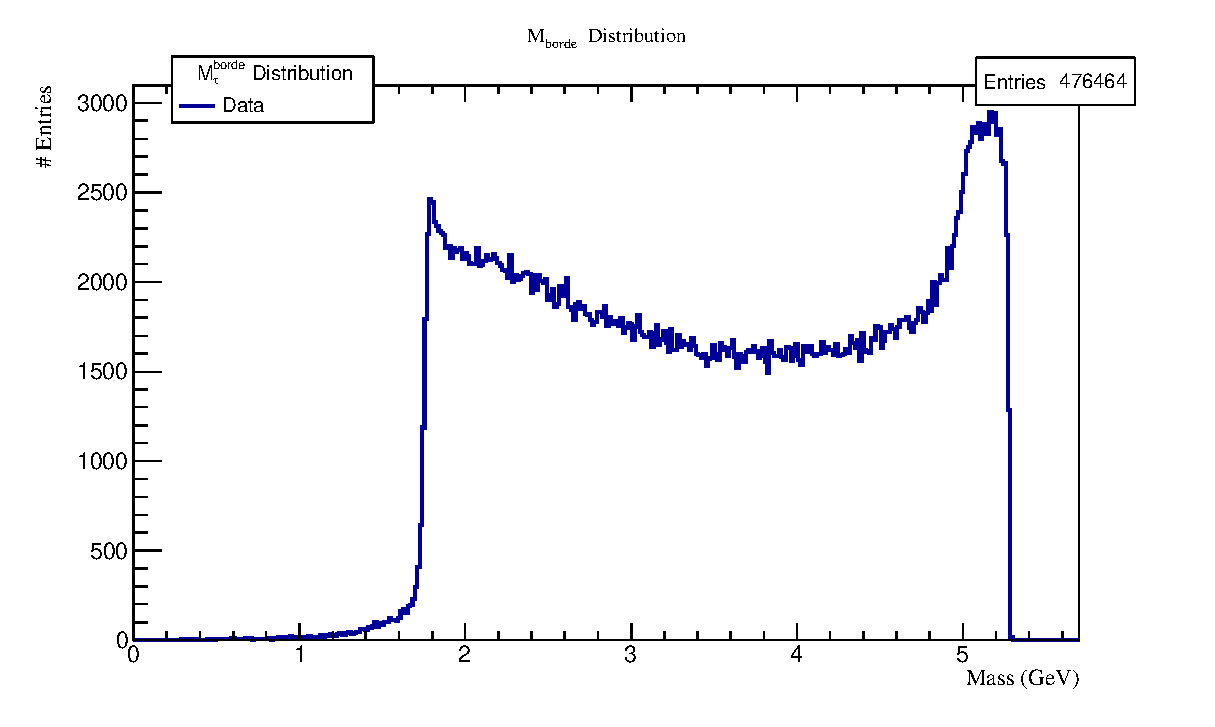
\includegraphics[width=\textwidth]{Images/m_edge_distri.eps} }}
      %\caption{Caption 1}
    \end{minipage}%
    \hfill
    \begin{minipage}[t]{0.56\textwidth}
      \centering
    \subfloat[\centering  ]{{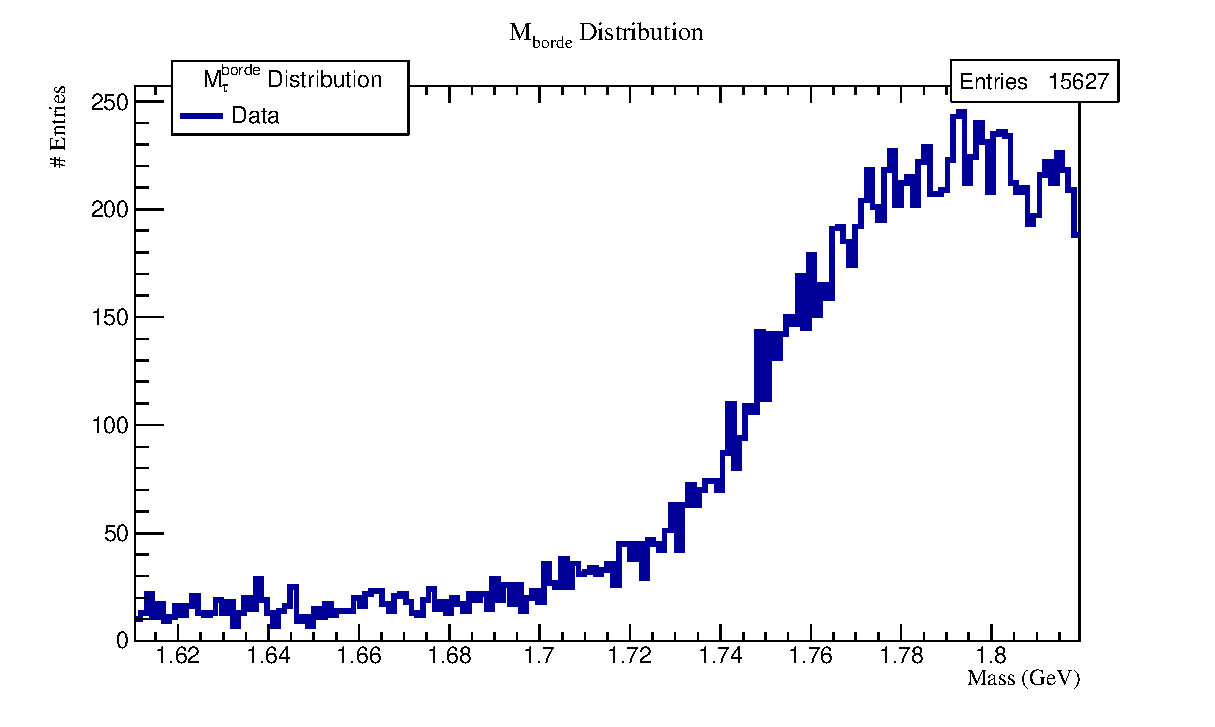
\includegraphics[width=\textwidth]{Images/m_edge_fit_distri.eps} }}
      %\caption{Caption 2}
    \end{minipage}%
  }%
  \caption{\small{(a) Distribución completa de la variable \(m^{borde}_{\tau}\) (sólo señal) de la muestra ``taupair'' de MC13a del experimento Belle II. (b) Distribución de la variable \(m^{borde}_{\tau}\) en la región de ajuste.}}
  \label{fig:mEdgeDistri}
\end{figure}
\begin{figure}[h]
    \centering
    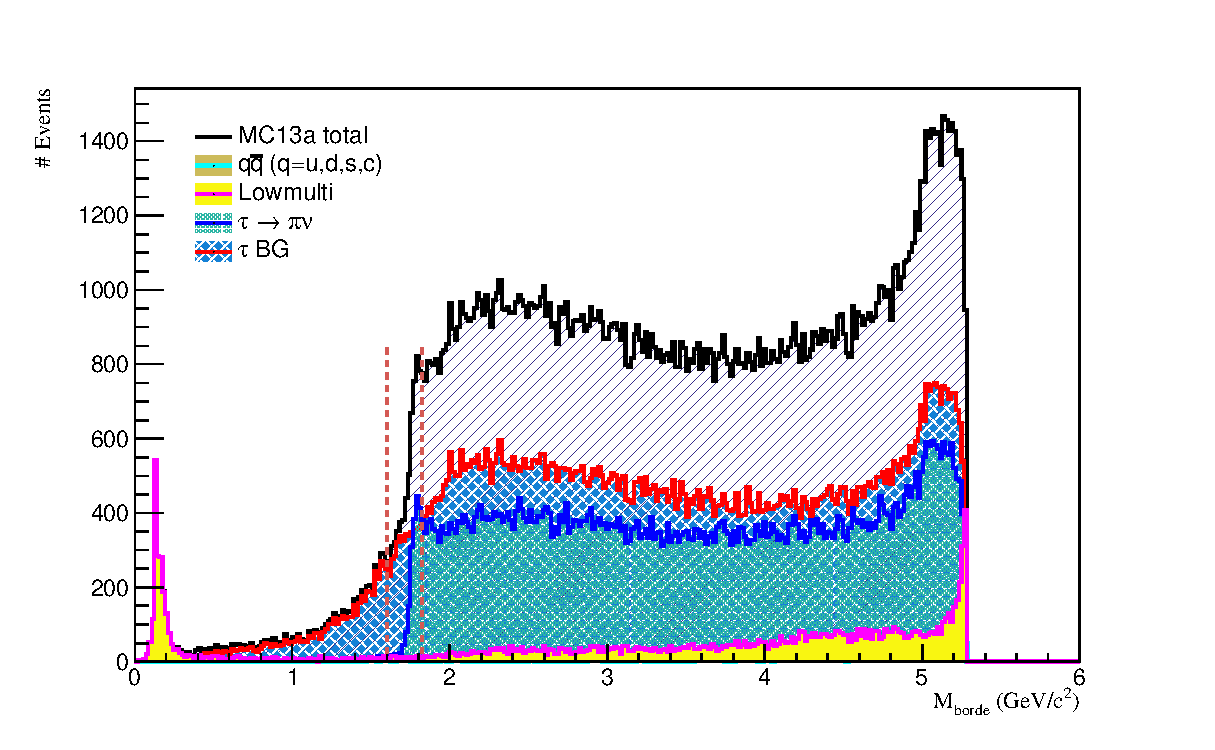
\includegraphics[scale=.6]{Images/m_edge_bdt_all.eps}
    \caption{\small{Distribución de \(m^{borde}_{\tau}\) MC13a con sus componentes de ruido y señal con corte en BDT>0.2. Distribución completa}}
    \label{fig:mEdgeBdtAll}
\end{figure} 
\begin{figure}[h]
    \centering
    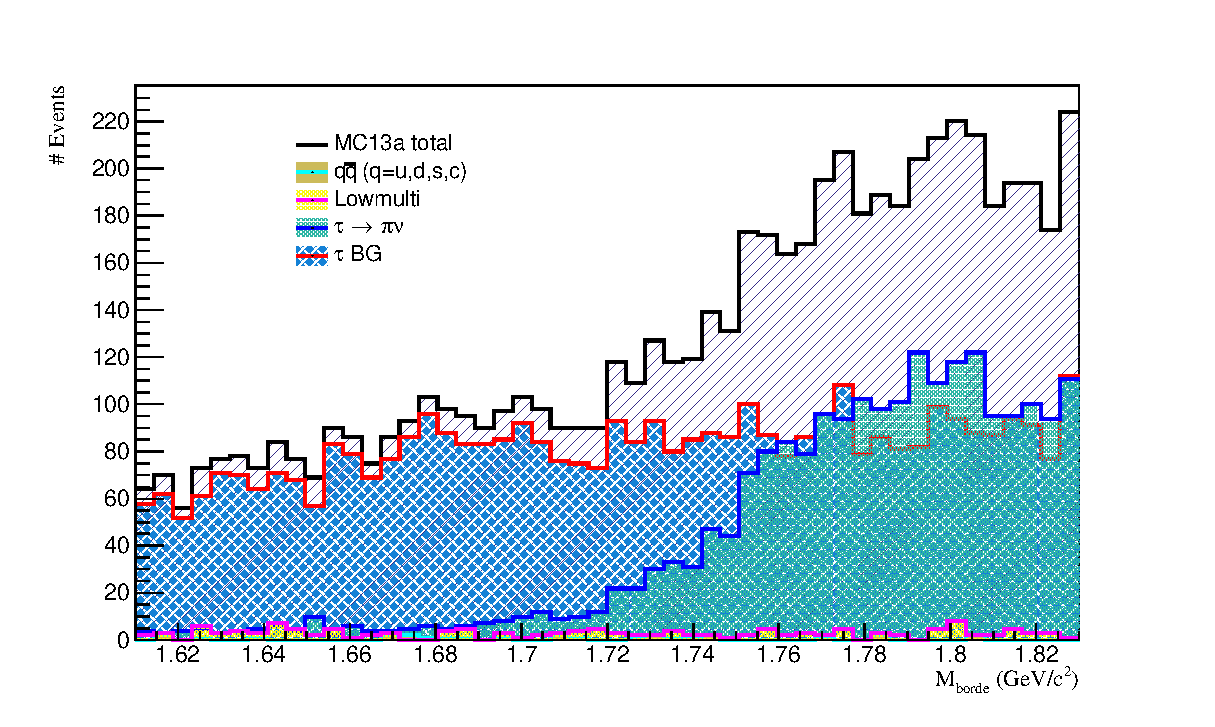
\includegraphics[scale=.6]{Images/m_edge_bdt_fit.eps}
    \caption{\small{Distribución de \(m^{borde}_{\tau}\) MC13a con sus componentes de ruido y señal con corte en BDT>0.2. Distribución en la región de ajuste.}}
    \label{fig:mEdgeFitBdtAllFit}
\end{figure} 


\chapter{Gráficos referentes a la variable \texorpdfstring{$M_{min}$}{TEXT}}

\begin{figure}[h]
  %\setcapwidth{0.6\textwidth}
  \checkoddpage
  \edef\side{\ifoddpage r\else l\fi}%
  \makebox[\textwidth][\side]{%
    \begin{minipage}[t]{0.56\textwidth}
      \centering
    \subfloat[\centering  ]{{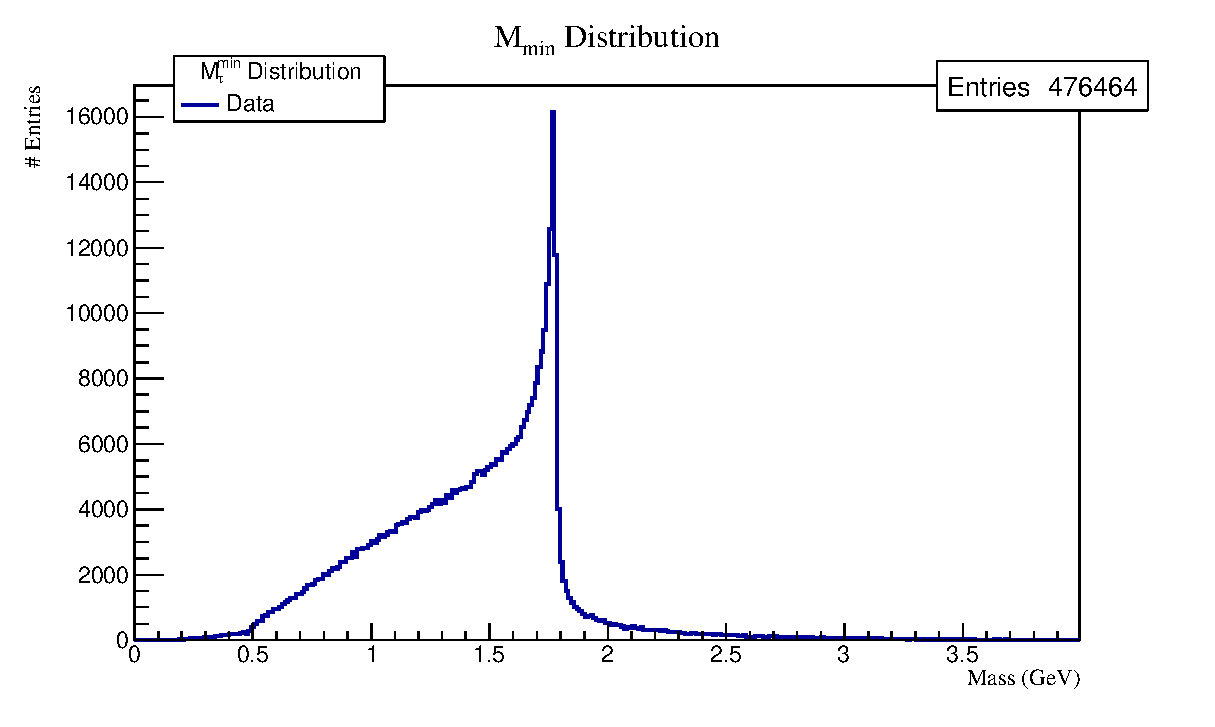
\includegraphics[width=\textwidth]{Images/m_min_complete.eps} }}
      %\caption{Caption 1}
    \end{minipage}%
    \hfill
    \begin{minipage}[t]{0.56\textwidth}
      \centering
    \subfloat[\centering  ]{{\includegraphics[width=\textwidth]{Images/m_min_fit_complete.eps} }}
      %\caption{Caption 2}
    \end{minipage}%
  }%
  \caption{\small{(a) Distribución completa de la variable \(m^{min}_{\tau}\) (sólo señal) de la muestra ``taupair'' de MC13a del experimento Belle II. (b) Distribución de la variable \(m^{min}_{\tau}\) en la región de ajuste.}}
  \label{fig:mMinDistri}
\end{figure}

\begin{figure}[h]
    \centering
    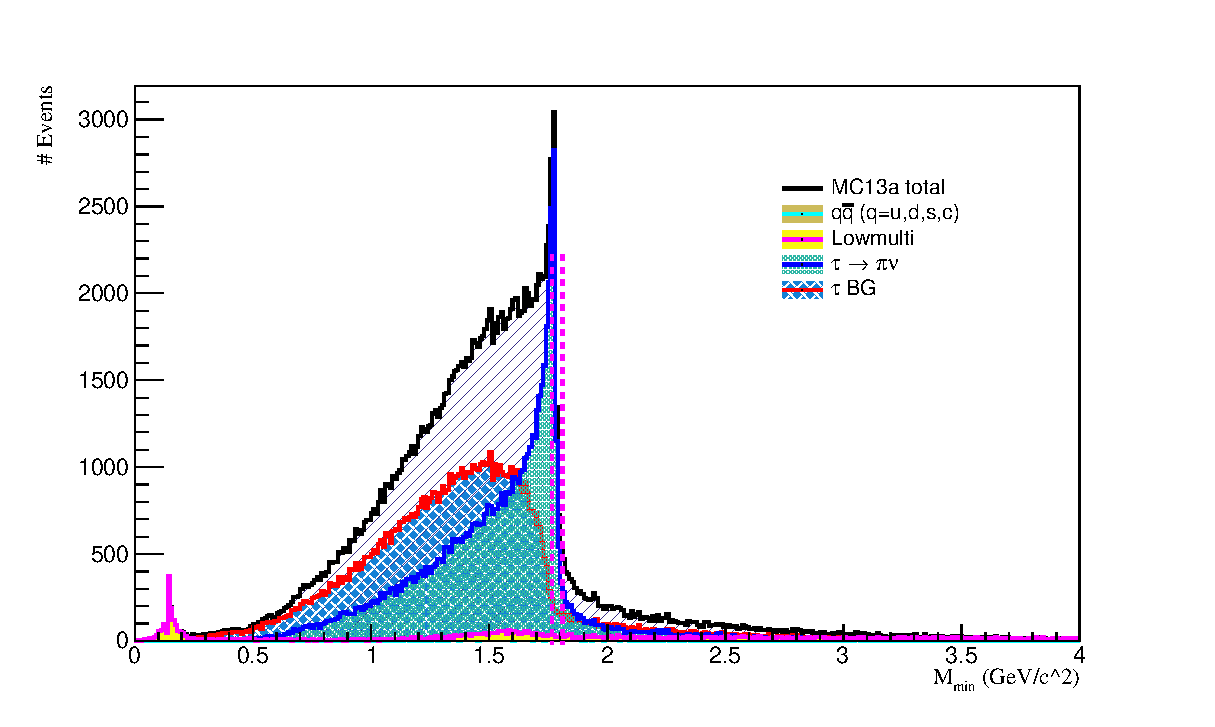
\includegraphics[scale=.6]{Images/m_min_plot_all.eps}
    \caption{\small{Distribución de \(m^{min}_{\tau}\) MC13a con sus componentes de ruido y señal con corte en BDT>0.2. Distribución completa}}
    \label{fig:mMinBdtAll}
\end{figure} 
\begin{figure}[h]
    \centering
    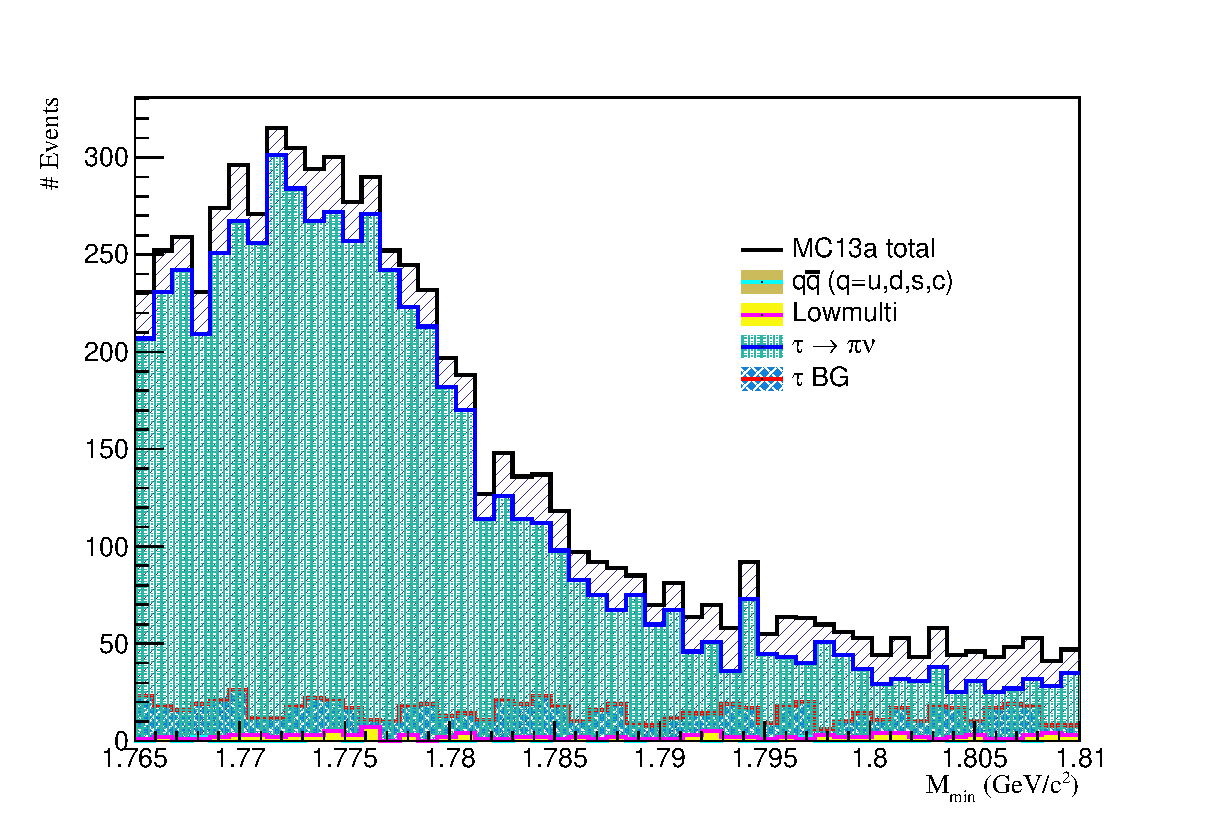
\includegraphics[scale=.6]{Images/m_min_fit_plot.eps}
    \caption{\small{Distribución de \(m^{min}_{\tau}\) MC13a con sus componentes de ruido y señal con corte en BDT>0.2. Distribución en la región de ajuste.}}
    \label{fig:mMinBdtAllFit}
\end{figure} 

 

\chapter{Gráficos referentes a la variable \texorpdfstring{$M_{max}$}{TEXT}}

\begin{figure}[h]
  %\setcapwidth{0.6\textwidth}
  \checkoddpage
  \edef\side{\ifoddpage r\else l\fi}%
  \makebox[\textwidth][\side]{%
    \begin{minipage}[t]{0.56\textwidth}
      \centering
    \subfloat[\centering  ]{{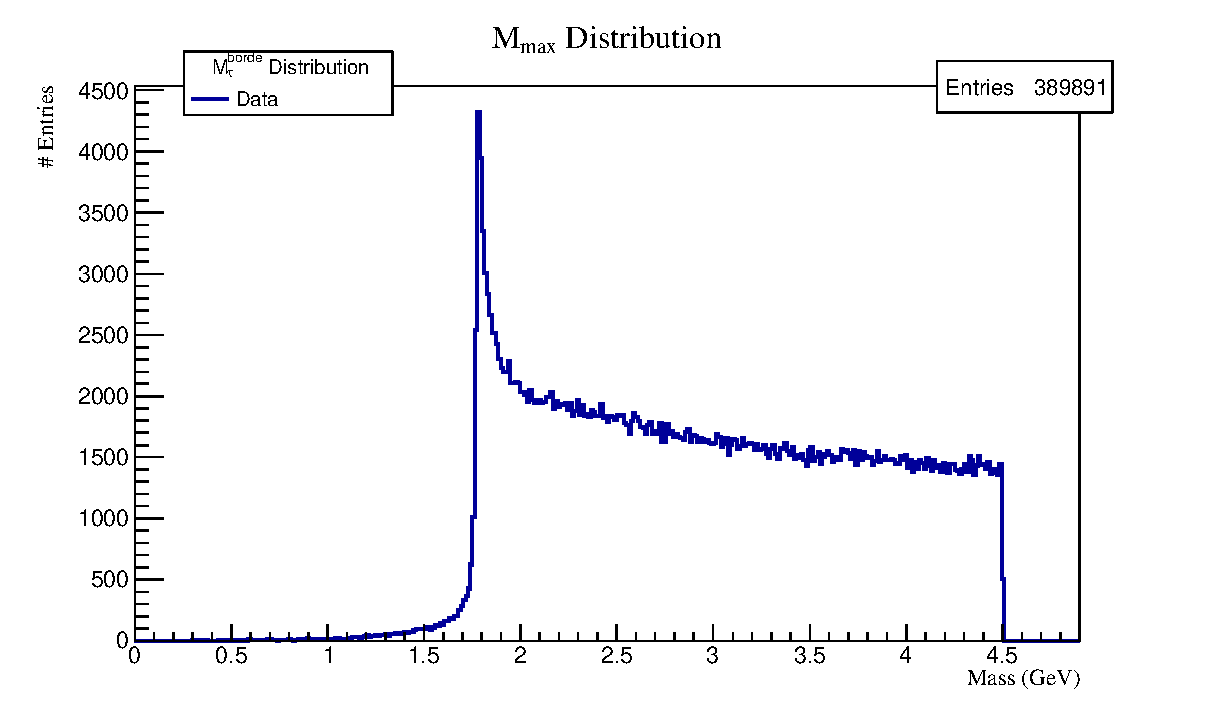
\includegraphics[width=\textwidth]{Images/m_max_distri.eps} }}
      %\caption{Caption 1}
    \end{minipage}%
    \hfill
    \begin{minipage}[t]{0.56\textwidth}
      \centering
    \subfloat[\centering  ]{{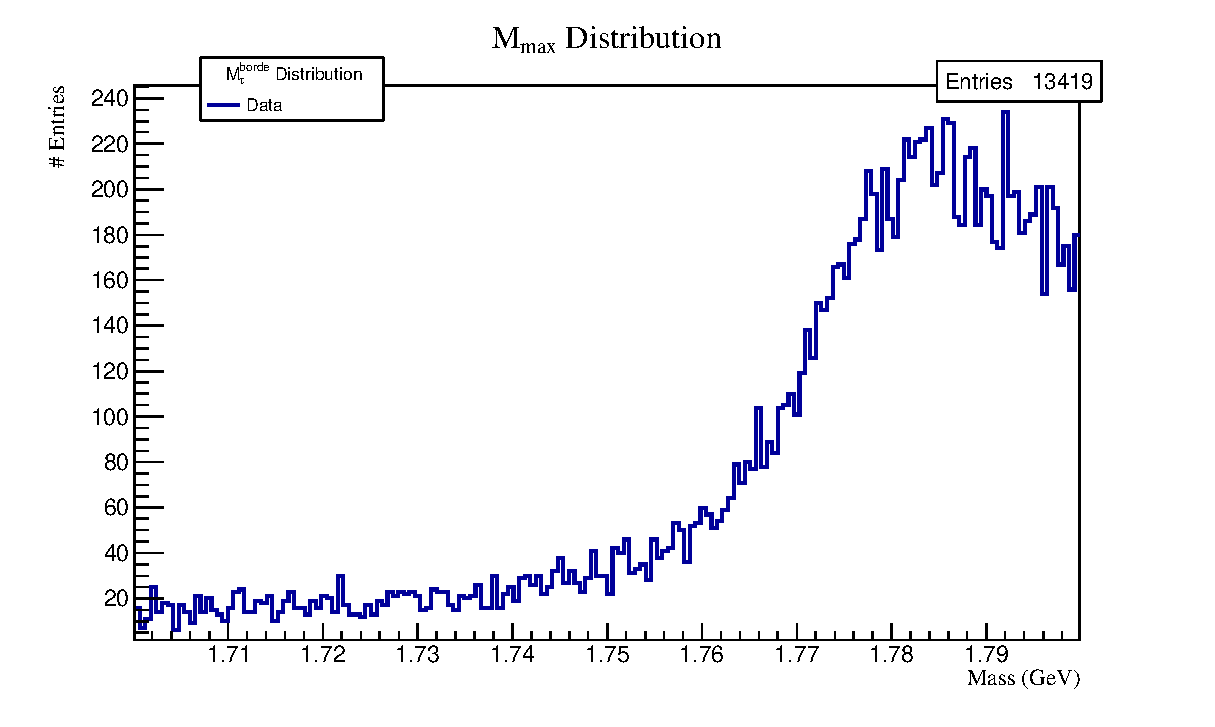
\includegraphics[width=\textwidth]{Images/m_max_distri_fit.eps} }}
      %\caption{Caption 2}
    \end{minipage}%
  }%
  \caption{\small{(a) Distribución completa de la variable \(m^{max}_{\tau}\) (sólo señal) de la muestra ``taupair'' de MC13a del experimento Belle II. (b) Distribución de la variable \(m^{max}_{\tau}\) en la región de ajuste.}}
  \label{fig:mMaxDistri}
\end{figure}
\begin{figure}[h]
    \centering
    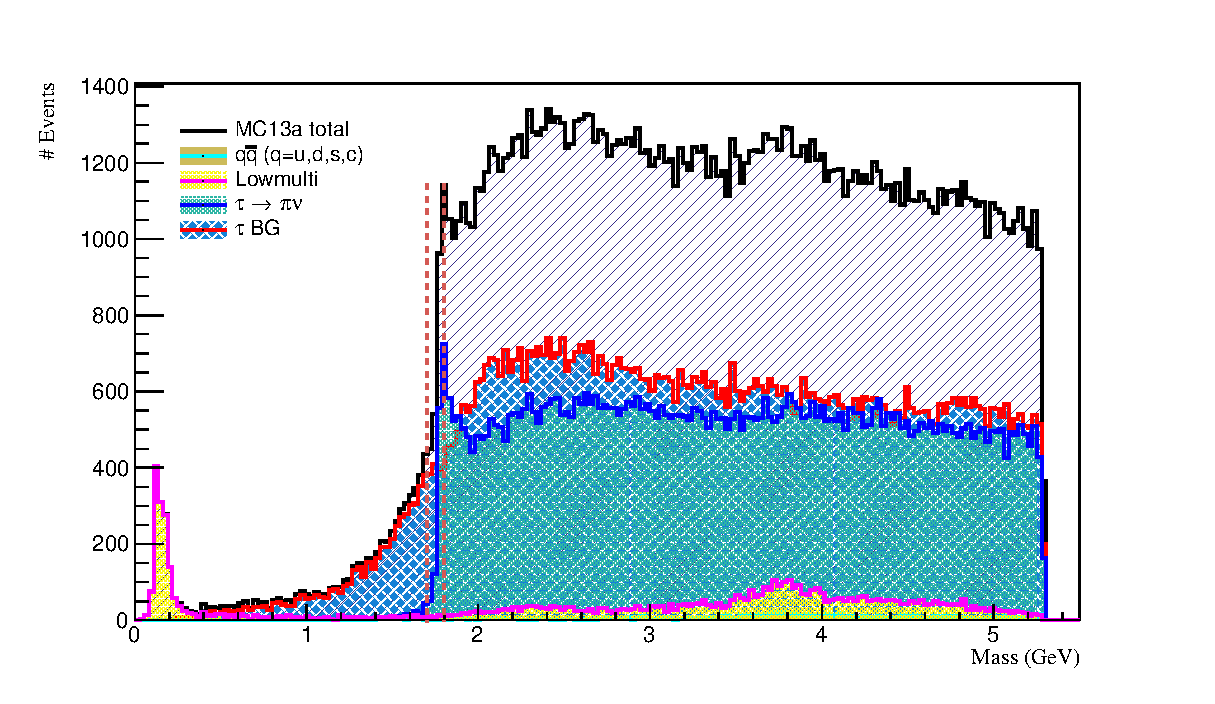
\includegraphics[scale=.6]{Images/m_max_plot_all.eps}
    \caption{\small{Distribución de \(m^{max}_{\tau}\) MC13a con sus componentes de ruido y señal con corte en BDT>0.2. Distribución completa}}
    \label{fig:mMaxBdtAll}
\end{figure} 
\begin{figure}[h]
    \centering
    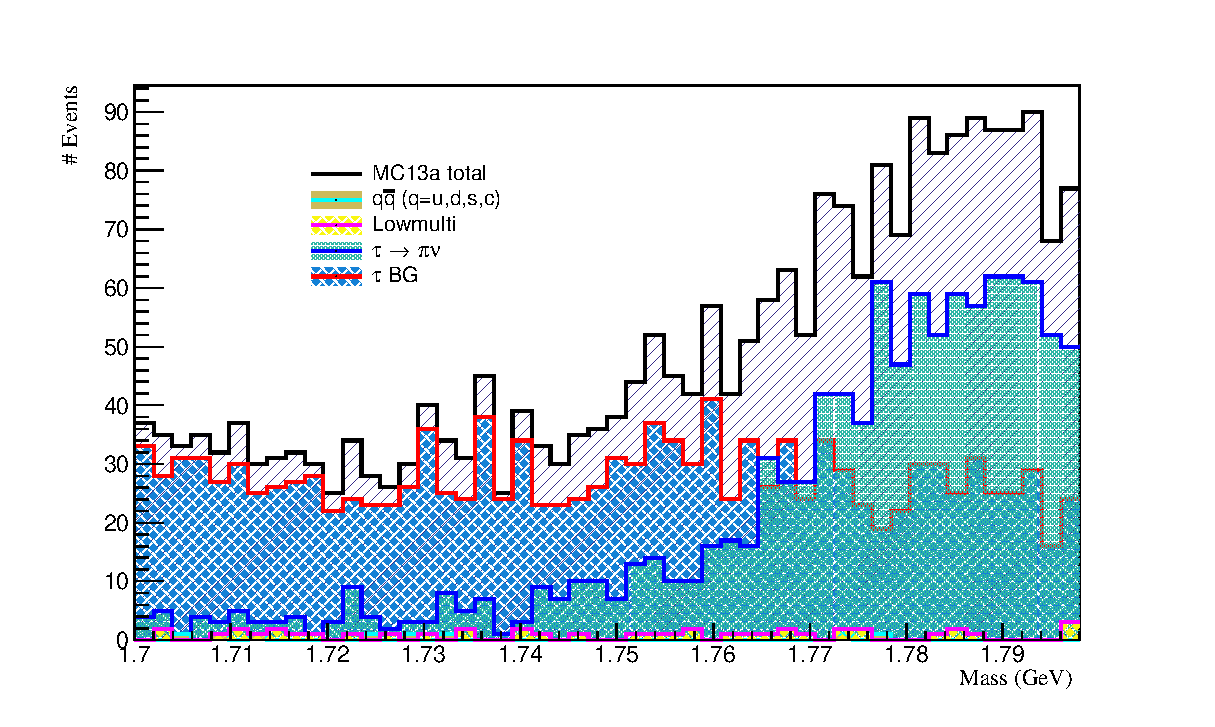
\includegraphics[scale=.6]{Images/m_max_fit_plot.eps}
    \caption{\small{Distribución de \(m^{max}_{\tau}\) MC13a con sus componentes de ruido y señal con corte en BDT>0.2. Distribución en la región de ajuste.}}
    \label{fig:mMaxBdtAllFit}
\end{figure} 

\end{appendices}